\documentclass{beamer}
\usepackage{ctex}
\usepackage{subfigure}
\usefonttheme[onlymath]{serif}
\CTEXoptions[today=old]
\usetheme{CambridgeUS}
\makeatletter
\renewcommand{\@thesubfigure}{\hskip\subfiglabelskip}
\makeatother
\usepackage{amsmath}
\DeclareSymbolFont{EulerExtension}{U}{euex}{m}{n}
\DeclareMathSymbol{\euintop}{\mathop} {EulerExtension}{"52}
\DeclareMathSymbol{\euointop}{\mathop} {EulerExtension}{"48}
\let\intop\euintop
\let\ointop\euointop
\usepackage{indentfirst}
\usepackage{ragged2e}
\begin{document}
\title{{\fangsong 基于PDE方法的一类图像去噪模型}}
\author{Author}
\institute{{\fangsong 吉林大学数学学院}}
\frame{\titlepage}

\begin{frame}{{\fangsong 研究背景}}

{\kaishu 图像在获取,存储及传输的过程中,通常会不可避免地受到各种
噪声的干扰,致使图像质量受到不同程度的损害。噪声会对图像产生不同
的影响,主要包括两个方面:}
\begin{itemize}
\item {\kaishu 影响主观视觉效果}
\item {\kaishu 无法继续对图像的信息层和知识层进行处理}
\end{itemize}
\end{frame}


\begin{frame}{{\fangsong 研究背景}}

\begin{footnotesize}
{\kaishu 近几年,基于偏微分方程(PDE)的图像去噪技术已经成为图
         像处理领域的强有力的工具。因其具有很强的自适应性,提高的变
通性和广泛的灵活性,其在图像处理和计算机视觉领域的诸多方面
已经有极为广泛的应用。

基本思想是将图像复原过程转化成球一个能量泛函模型或一系列PDE,以待处理图像作为方程初始值,经过数值迭代或智能优化的方法对该过程求解,最后得到的方程解即是需要的处理结果。这种算法的优势主要体现在以下四个方面:}
\begin{itemize}
\item {\kaishu 能够在连续领域中进行图像处理,大大简化了图像复原问题}
\item {\kaishu 能够直接利用图像的几何特征分析图像,比如:曲率,水平集,梯度和切线等}
\item {\kaishu 能够很好的模拟人类视觉意义的各同向性和各向异性扩散方程}
\item {\kaishu 可以直接通过成熟的数值计算方法,或利用优化智能方法进行数值实现}
\end{itemize}
\end{footnotesize}
\end{frame}
\begin{frame}{{\fangsong 国内外研究现状}}
\begin{footnotesize}
\begin{itemize}
\item {\kaishu 基于PDE的理论最早可以追溯到1965年Gabor以及后来Jain等人关于图像光滑和图像增强的研究工作}
\item {\kaishu 1983年和1984年,Koenderink和Witkin引入了尺度空间的严格理论,并明确指出了高斯滤波,处理过程中与热传导方程的各向同性扩散过程是等效的}
\item {\kaishu 1990年,Rudin,Oshen和Fatemi提出了另一个著名的图像去噪模型,即TV 模型。提出运用ROF方法即使用人工时间演化求解欧拉方程,又称为ROF模型}
\item {\kaishu 2000年,You Y L等人提出了一种四阶PDE 模型,在此过程中PDE去噪方法实现了从低阶到高阶的过渡}
\item {\kaishu 2008年,Chen Y 等人提出了一种改进的四阶图像去噪模型}
\end{itemize}
\end{footnotesize}
\end{frame}
\begin{frame}{{\fangsong 主要工作}}
\begin{itemize}
\item {\kaishu 分析了Chen Y, Vrmuri B C和 Wang L等人的一类PDE模型, 进而给出了模型的一种改进形式}
\item {\kaishu 对模型进行了数值实现,从数学角度分析了其可行性和有效性}
\item {\kaishu 对模型进行仿真试验和结果分析}
\end{itemize}
\end{frame}
\begin{frame}{{\fangsong PDE图像去噪 数学理论及方法}}
\begin{itemize}
\item {\kaishu 变分方法的能量极小化原理}
\item {\kaishu 泛函、变分原理及梯度下降流}
\item {\kaishu 有限差分法}
\end{itemize}
\end{frame}
\begin{frame}{{\fangsong 模型的提出}}
\begin{footnotesize}
{\kaishu 文献[1]能量泛函}
$$E(u)=\iint_{\varOmega}\{g(\nabla G*u)|\nabla u|+\beta(u-I)^{2}\}\mathrm{d}x\mathrm{d}y$$

{\kaishu 对应的梯度流方程}
$$\frac{\partial u}{\partial t}=-E'(u)$$

{\kaishu 文献[1]修正以上梯度流方程为:}
$$\frac{\partial u}{\partial t}=-|\nabla u|\cdot E'(u)$$

{\kaishu 得到用于处理图像去噪的偏微分模型:}
\begin{scriptsize}
\begin{equation}
\left\{
\begin{aligned}
&\frac{\partial u}{\partial t}=  g(\nabla G_{\sigma}*u)|\nabla u|\mathrm{div}\left(\frac{\nabla u}{|\nabla u|}\right)+\nabla g(\nabla G_{\sigma}*u)\cdot\nabla u-\beta|\nabla u|(u-I), x\in\varOmega,t>0\\
&u(x,0) =I(x),x\in\varOmega
\end{aligned}
\right.
\end{equation}
\end{scriptsize}
\end{footnotesize}
\end{frame}
\begin{frame}{{\fangsong 模型的改进}}
\begin{footnotesize}
{\kaishu 在本文中,基于上述两者梯度流方程,使用下面的梯度流方程:}
$$\frac{\partial u}{\partial t}=-\frac{|\nabla u|}{\theta+|\nabla u|^{1-\theta}}\cdot E'(u)$$

{\kaishu 其中$0<\theta\leq 1$。当$\theta=1$时,这个模型与文献[1]的模型是一样的,当$\theta\rightarrow 0$时,该方程在形式上趋于未修正的梯度流方程。从这里可以看出,本文中的模型要比文献[1]中的模型更广泛,更具有一般意义。}

{\kaishu 根据以上修正的梯度流方程,得到相应的初值问题:}
\begin{tiny}
\begin{equation}
\left\{
\begin{aligned}
&\frac{\partial u}{\partial t}=  \frac{1}{\theta+|\nabla u|^{1-\theta}}\{g(\nabla G_{\sigma}*u)|\nabla u|\mathrm{div}\left(\frac{\nabla u}{|\nabla u|}\right)+\nabla g(\nabla G_{\sigma}*u)\cdot\nabla u-\beta|\nabla u|(u-I)\}, x\in\varOmega,t>0\\
&u(x,0) =I(x),x\in\varOmega
\end{aligned}
\right.
\end{equation}
\end{tiny}
\end{footnotesize}
\end{frame}
\begin{frame}{{\fangsong 模型的改进}}

{\kaishu 根据之前的算法,我们可以得到方程(2)的差分格式为:}
\begin{scriptsize}
$$\frac{u^{n+1}(i,j)-u^{n}(i,j)}{\tau}=g(u^{n}(i,j))l(u^{n}(i,j))+\nabla g\cdot\nabla u^{n}(i,j)-|\nabla u^{n}|(i,j)(u^{n}(i,j)-I(i,j))$$
\end{scriptsize}
\end{frame}
\begin{frame}{\fangsong 实验结果及分析}
\begin{footnotesize}
{\kaishu 本文将模型 (1) 和模型 (2) 的实验结果进行了比较,实验证明本文提出的模型 (2) 具有
更好的去噪效果。}

{\kaishu 本文通过第二部分所介绍的相关理论和方法,通过变分原理,对图像能量泛函的极小值
问题进行了分析,在已有的模型基础上,提出了一类改进的 PDE 去噪模型。改进的模型主
要是考虑到之前的两类偏微分模型的联系,在此基础上再梯度流方程中乘以不同的系数项,
这样的话使该种模型具有更好地去噪效果。实验结果证明,利用改进后的模型不但对图像边
缘有更佳良好的保护效果,而且背景物体以及图像的主体也更加细致清晰,因此可以得到比
较理想的去噪效果。}

\end{footnotesize}
\end{frame}
\begin{frame}{\fangsong 实验结果及分析}
\begin{figure}[!h]
\begin{footnotesize}
\centering
\subfigure[{\scriptsize\kaishu 初始图像}]{
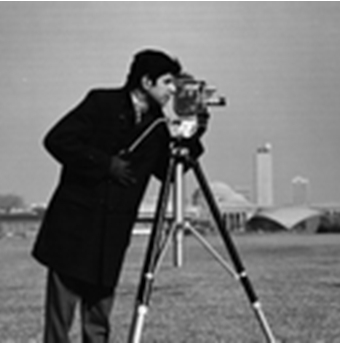
\includegraphics[width=2.7cm]{1.png}
}
\quad
\subfigure[{\scriptsize\kaishu 加噪图像}]{
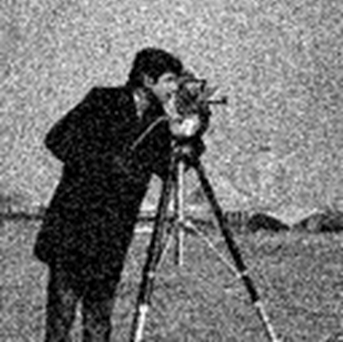
\includegraphics[width=2.7cm]{2.png}
}

\subfigure[{\scriptsize\kaishu 模型(1)结果图像}]{
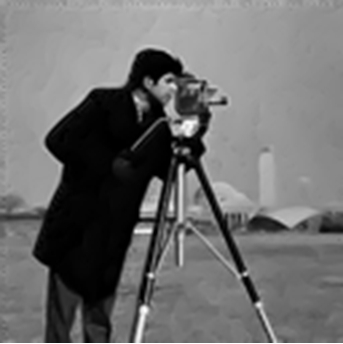
\includegraphics[width=2.7cm]{3.png}
}
\quad
\subfigure[{\scriptsize\kaishu 模型(2)结果图像}]{
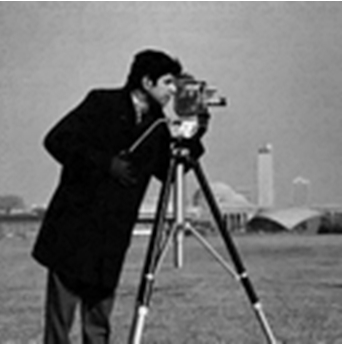
\includegraphics[width=2.7cm]{4.png}
}
\end{footnotesize}
\end{figure}
\end{frame}
\end{document}
